% SQLChange — Agentic SQL Query Optimization Pipeline
% UC Davis Beamer template (Aggie Blue / Gold)
% Compiles with pdfLaTeX.

\documentclass[10pt,aspectratio=169]{beamer}

% ====================
% Packages
% ====================
\usepackage[T1]{fontenc}
\usepackage{lmodern}
\usepackage{graphicx}
\usepackage{booktabs}
\usepackage{mathtools}
\usepackage{tikz}
\usetikzlibrary{positioning,arrows.meta,shapes.geometric,calc,backgrounds}
\usepackage{hyperref}
\usepackage{pgfplots}
\pgfplotsset{compat=1.18}

% ====================
% UC Davis brand colors (digital palette)
% ====================
\definecolor{aggieblue}{HTML}{022851}
\definecolor{aggiegold}{HTML}{FFBF00}
\definecolor{aggieblueDark}{HTML}{011936}
\definecolor{aggiegoldDark}{HTML}{C99700}
\definecolor{coolgray}{RGB}{77,79,83}
\definecolor{boxgray}{RGB}{238,235,233}

% ====================
% Fonts
% ====================
\renewcommand{\familydefault}{\sfdefault}
\newcommand{\Raleway}{\sffamily}
\newcommand{\Lato}{\sffamily}

% ====================
% Beamer color slots
% ====================
\setbeamercolor*{palette primary}{fg=white,bg=aggieblue}
\setbeamercolor*{palette secondary}{fg=white,bg=coolgray}
\setbeamercolor*{palette tertiary}{fg=white,bg=aggieblueDark}
\setbeamercolor*{palette quaternary}{fg=aggieblue,bg=aggiegold}

\setbeamercolor{structure}{fg=aggieblue}
\setbeamercolor{titlelike}{fg=aggieblue}
\setbeamercolor{frametitle}{fg=white,bg=aggieblue}
\setbeamercolor{title}{fg=white,bg=aggieblue}
\setbeamercolor{author}{fg=aggieblue}
\setbeamercolor{institute}{fg=coolgray}
\setbeamercolor{date}{fg=coolgray}

\setbeamercolor{section in toc}{fg=aggieblue}
\setbeamercolor{subsection in toc}{fg=aggieblueDark}

% ====================
% Fonts (sizes/weights)
% ====================
\setbeamerfont{title}{family=\Raleway,series=\bfseries,size=\LARGE}
\setbeamerfont{subtitle}{family=\Lato,size=\normalsize}
\setbeamerfont{author}{family=\Lato,size=\small}
\setbeamerfont{institute}{family=\Lato,size=\footnotesize}
\setbeamerfont{date}{family=\Lato,size=\footnotesize}
\setbeamerfont{frametitle}{family=\Raleway,series=\bfseries,size=\large}
\setbeamerfont{section in toc}{family=\Raleway,series=\bfseries}
\setbeamerfont{subsection in toc}{family=\Lato,size=\small}
\setbeamerfont{footline}{family=\Lato,size=\scriptsize}

% ====================
% Frame title with Aggie Gold accent bar
% ====================
\setbeamertemplate{frametitle}{%
  \nointerlineskip
  \begin{beamercolorbox}[wd=\paperwidth,ht=3.0ex,dp=1.4ex,leftskip=1em,rightskip=1em]{frametitle}%
    \usebeamerfont{frametitle}\insertframetitle%
  \end{beamercolorbox}%
  \begin{beamercolorbox}[wd=\paperwidth,ht=0.35ex,dp=0pt]{palette quaternary}%
  \end{beamercolorbox}%
  \vspace{1.0ex}
}

\beamertemplatenavigationsymbolsempty

% ====================
% Table of Contents Customization
% ====================
\setbeamertemplate{section in toc}{\leavevmode\inserttocsection\par}

\setbeamertemplate{subsection in toc}{%
  \leavevmode\hspace{1.5em}%
  \color{aggiegoldDark}\raise0.4ex\hbox{\vrule width 0.4ex height 0.4ex}%
  \hspace{0.5em}\color{aggieblueDark}\inserttocsubsection\par
}

% ====================
% Footer
% ====================
\newcommand{\footercontent}[1]{\renewcommand{\insertfootercontent}{#1}}
\newcommand{\insertfootercontent}{}

\setbeamertemplate{footline}{%
  \ifx\insertfootercontent\@empty\else
    \begin{beamercolorbox}[wd=\paperwidth,ht=0.3ex,dp=0pt]{palette quaternary}\end{beamercolorbox}%
    \begin{beamercolorbox}[wd=\paperwidth,ht=2.4ex,dp=1.2ex,leftskip=1em,rightskip=1em]{palette primary}%
      \usebeamerfont{footline}\insertfootercontent\hfill\insertframenumber{}/\inserttotalframenumber%
    \end{beamercolorbox}%
  \fi
}

% ====================
% Title / authors
% ====================
\title{SQLChange: Agentic SQL Query Optimization}
\subtitle{}
\author{Ahmed Khan \and Fahim Islam \and Dev Rathod \and Arnav Akula \and Devarchith Parashara Batchu}
\institute{Department of Computer Science \\ University of California, Davis}
\date{\today}

\titlegraphic{}

\footercontent{%
  \href{https://github.com/FahimIslam731/SQLChange}{github.com/FahimIslam731/SQLChange}
  \enspace$\bullet$\enspace
  UC Davis --- ECS 271%
}

% ====================
% Title page template
% ====================
\setbeamertemplate{title page}{%
  \begin{tikzpicture}[remember picture,overlay]
    \fill[aggieblue]
      ([yshift=1cm]current page.north west)
      rectangle
      ([yshift=-3.8cm]current page.north east);
    \fill[aggiegold]
      ([yshift=-3.8cm]current page.north west)
      rectangle
      ([yshift=-3.95cm]current page.north east);
    \node[anchor=center,text=white,align=center,text width=14cm,
          font=\Raleway\bfseries]
      at ([yshift=-2.2cm]current page.north)
      {\usebeamerfont{title}\inserttitle};
    \node[anchor=center,text=aggiegold,align=center,text width=14cm,
          font=\Lato]
      at ([yshift=-2.4cm]current page.north)
      {\usebeamerfont{subtitle}\insertsubtitle};
    \node[anchor=north,text=aggieblue,align=center,font=\Lato]
      at ([yshift=-5.4cm]current page.north)
      {\usebeamerfont{author}\insertauthor};
    \node[anchor=north,text=coolgray,align=center,font=\Lato]
      at ([yshift=-6.0cm]current page.north)
      {\usebeamerfont{institute}\insertinstitute};
    \node[anchor=north,text=coolgray,align=center,font=\Lato]
      at ([yshift=-6.9cm]current page.north)
      {\usebeamerfont{date}\insertdate};
  \end{tikzpicture}%
}

% ====================
% Section declarations (populate the TOC)
% ====================
\section{Motivation}
\section{Pipeline Architecture}
\subsection{Parsing \& Schema Inference}
\subsection{ER Graph Construction}
\subsection{LLM Recommendation Engine}
\subsection{Execution Harness}
\subsection{Reasoning \& Labeling}
\subsection{Iterative Feedback Loop}
\section{Evaluation}
\subsection{Dataset}
\subsection{Results}
\section{Demo}
\section{Conclusion \& Future Work}


% ====================
% Document
% ====================
\begin{document}

% ---------- Title Slide ----------
{%
  \setbeamertemplate{footline}{}%
  \begin{frame}[plain,noframenumbering]
    \titlepage
  \end{frame}
}

% ---------- Table of Contents ----------
\begin{frame}{Contents}
  \tableofcontents
\end{frame}

% ==========================================================================
% MOTIVATION
% ==========================================================================

\begin{frame}{Motivation}
  \begin{columns}[T]

    \begin{column}{0.55\textwidth}
      \begin{large}
      \begin{itemize}
        \setlength{\itemsep}{1.0em}
        \item SQL optimization requires \textbf{deep expertise} in query plans, indexing, and schema design
        \item Manual review is \textbf{slow, error-prone}, and doesn't scale
        \item Existing tools suggest changes but \textbf{don't verify} equivalence or safety
      \end{itemize}
      \end{large}

      \vspace{1.0em}

      \setbeamercolor{boxblue}{bg=aggieblue,fg=white}
      \begin{beamercolorbox}[wd=\textwidth,rounded=true,leftskip=0.7em,rightskip=0.7em,sep=0.6em]{boxblue}
        \small\Lato\bfseries\color{white}
        SQLChange: an agentic LangGraph pipeline that parses, optimizes, and \textit{execution-verifies} SQL queries using LLMs and synthetic databases
      \end{beamercolorbox}
    \end{column}

    \begin{column}{0.42\textwidth}
      \centering
      \vspace{0.5em}
      {\small\Raleway\bfseries\color{aggieblue} Three Interfaces}\\[0.6em]
      \begin{beamercolorbox}[wd=\textwidth,rounded=true,shadow=false,sep=0.4em]{boxgray}
        \usebeamerfont{footline}\color{coolgray}
        \centering{\textbf{\color{aggieblue}CLI}}\\[0.2em]
        \scriptsize\texttt{python cli.py --interactive}\\
        Step-by-step debug output
      \end{beamercolorbox}
      \vspace{0.3em}
      \begin{beamercolorbox}[wd=\textwidth,rounded=true,shadow=false,sep=0.4em]{boxgray}
        \usebeamerfont{footline}\color{coolgray}
        \centering{\textbf{\color{aggieblue}REST API}}\\[0.2em]
        \scriptsize\texttt{POST /optimize}\\
        JSON in, JSON out
      \end{beamercolorbox}
      \vspace{0.3em}
      \begin{beamercolorbox}[wd=\textwidth,rounded=true,shadow=false,sep=0.4em]{boxgray}
        \usebeamerfont{footline}\color{coolgray}
        \centering{\textbf{\color{aggieblue}Python API}}\\[0.2em]
        \scriptsize\texttt{run\_pipeline(sql, ddl, ...)}\\
        Programmatic integration
      \end{beamercolorbox}
    \end{column}

  \end{columns}
\end{frame}

% ==========================================================================
% PIPELINE ARCHITECTURE
% ==========================================================================

% ---------- Transition Slide ----------
{%
  \setbeamertemplate{footline}{}%
  \begin{frame}[plain,noframenumbering]
    \begin{tikzpicture}[remember picture,overlay]
      \fill[aggieblue] (current page.south west) rectangle (current page.north east);
    \end{tikzpicture}
    \vfill
    \centering
    {\Raleway\bfseries\Huge\color{white} Pipeline Architecture}\\[0.6em]
    {\color{aggiegold}\rule{6cm}{0.06cm}}
    \vfill
  \end{frame}
}

% ---------- Pipeline Overview ----------
\begin{frame}{Pipeline Overview}
  \centering
  \vspace{-0.4em}
  \resizebox{0.97\textwidth}{!}{%
  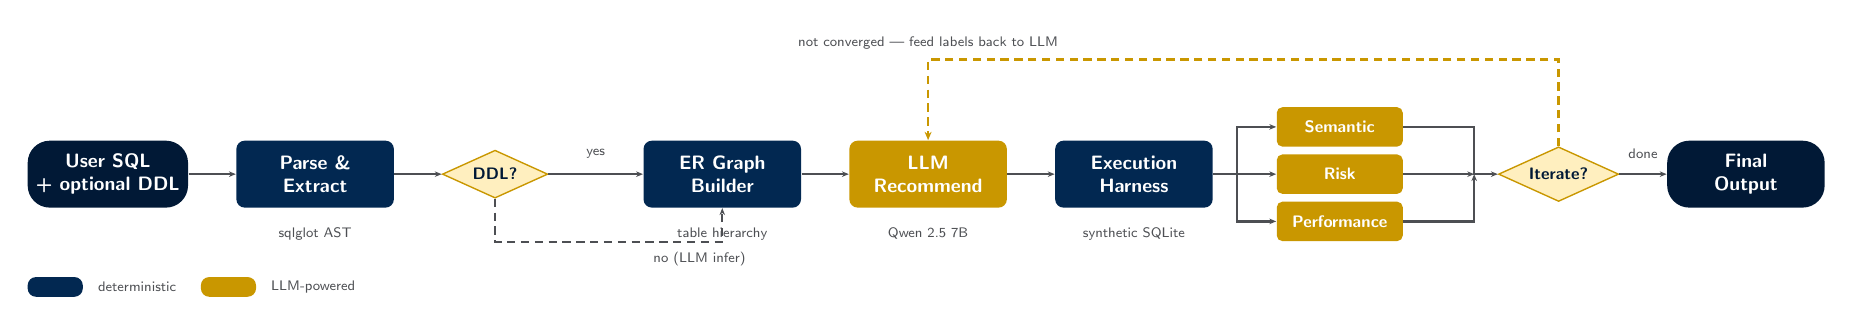
\begin{tikzpicture}[
    node distance=0.4cm and 0.6cm,
    % --- Node styles ---
    stage/.style={
      rectangle, rounded corners=3pt,
      minimum height=0.85cm, minimum width=2.0cm,
      font=\fontsize{7}{8.5}\selectfont\bfseries,
      align=center, inner sep=3pt, draw=none,
    },
    determ/.style={stage, fill=aggieblue, text=white},
    llmnode/.style={stage, fill=aggiegoldDark, text=white},
    iobox/.style={stage, fill=aggieblueDark, text=white, rounded corners=8pt},
    decision/.style={
      diamond, aspect=2.2,
      minimum height=0.6cm, minimum width=0.9cm,
      font=\fontsize{6}{7}\selectfont\bfseries,
      fill=aggiegold!25, draw=aggiegoldDark, line width=0.5pt,
      text=aggieblueDark, inner sep=2pt, align=center,
    },
    sublabel/.style={
      rectangle, rounded corners=2pt,
      minimum height=0.5cm, minimum width=1.6cm,
      font=\fontsize{6}{7}\selectfont\bfseries,
      inner sep=2pt, align=center, draw=none,
    },
    % --- Arrow styles ---
    flow/.style={-{Stealth[length=2.5pt, width=2pt]}, thick, color=coolgray},
    branchflow/.style={flow, densely dashed},
    loopback/.style={-{Stealth[length=3pt, width=2.5pt]}, thick, color=aggiegoldDark, densely dashed},
    % --- Annotation style ---
    annot/.style={font=\fontsize{5}{6}\selectfont, text=coolgray, align=center},
  ]

    % ===================== MAIN CHAIN =====================
    \node[iobox]                          (input) {User SQL\\+ optional DDL};
    \node[determ, right=of input]         (parse) {Parse \&\\Extract};
    \node[decision, right=0.6cm of parse] (ddl)   {DDL?};
    \node[determ, right=1.2cm of ddl]     (er)    {ER Graph\\Builder};
    \node[llmnode, right=of er]           (rec)   {LLM\\Recommend};
    \node[determ, right=of rec]           (exec)  {Execution\\Harness};

    % ===================== LABELER FAN-OUT =====================
    \node[sublabel, fill=aggiegoldDark, text=white,
          right=0.8cm of exec, yshift=0.6cm]    (lsem)  {Semantic};
    \node[sublabel, fill=aggiegoldDark, text=white,
          right=0.8cm of exec]                   (lrisk) {Risk};
    \node[sublabel, fill=aggiegoldDark, text=white,
          right=0.8cm of exec, yshift=-0.6cm]   (lperf) {Performance};

    % ===================== ITERATION DECISION =====================
    \node[decision, right=0.8cm of lrisk, xshift=0.4cm] (iter) {Iterate?};
    \node[iobox, right=0.6cm of iter]                    (out)  {Final\\Output};

    % ===================== ARROWS: MAIN FLOW =====================
    \draw[flow] (input) -- (parse);
    \draw[flow] (parse) -- (ddl);

    % DDL yes branch (straight through)
    \draw[flow] (ddl.east) -- (er)
      node[annot, midway, above, yshift=2pt] {yes};

    % DDL no branch (dip below, label on the horizontal segment)
    \draw[branchflow] (ddl.south) -- ++(0,-0.55)
      -| (er.south)
      node[annot, pos=0.45, below] {no (LLM infer)};

    \draw[flow] (er) -- (rec);
    \draw[flow] (rec) -- (exec);

    % Fan-out to labelers
    \coordinate (fanpt) at ($(exec.east)+(0.3,0)$);
    \draw[flow] (exec.east) -- (fanpt) |- (lsem.west);
    \draw[flow] (fanpt) -- (lrisk.west);
    \draw[flow] (fanpt) |- (lperf.west);

    % Labelers converge to iteration decision
    \coordinate (convpt) at ($(iter.west)+(-0.3,0)$);
    \draw[flow] (lsem.east)  -| (convpt) -- (iter.west);
    \draw[flow] (lrisk.east) -- (convpt);
    \draw[flow] (lperf.east) -| (convpt);

    % Iterate? -> done
    \draw[flow] (iter.east) -- (out)
      node[annot, midway, above, yshift=2pt] {done};

    % ===================== FEEDBACK LOOP =====================
    \draw[loopback]
      (iter.north) -- ++(0,1.1)
      -| (rec.north)
      node[annot, pos=0.5, above] {not converged --- feed labels back to LLM};

    % ===================== ANNOTATIONS BELOW NODES =====================
    \node[annot, below=0.12cm of parse]  {sqlglot AST};
    \node[annot, below=0.12cm of er]     {table hierarchy};
    \node[annot, below=0.12cm of rec]    {Qwen 2.5 7B};
    \node[annot, below=0.12cm of exec]   {synthetic SQLite};

    % ===================== LEGEND (bottom-left, below annotations) =====================
    \begin{scope}[shift={($(input.south west)+(0,-1.0)$)}]
      \node[determ, minimum width=0.7cm, minimum height=0.25cm,
            font=\fontsize{4}{5}\selectfont, anchor=west] (ld) at (0,0) {};
      \node[annot, anchor=west] at (ld.east) {~deterministic};
      \node[llmnode, minimum width=0.7cm, minimum height=0.25cm,
            font=\fontsize{4}{5}\selectfont, anchor=west] (ll) at (2.2,0) {};
      \node[annot, anchor=west] at (ll.east) {~LLM-powered};
    \end{scope}

  \end{tikzpicture}%
  }% end resizebox

  \vspace{0.6em}

  \begin{columns}[T, onlytextwidth]
    \begin{column}{0.30\textwidth}
      \begin{beamercolorbox}[wd=\textwidth,rounded=true,shadow=false,sep=0.4em]{boxgray}
        \usebeamerfont{footline}\color{coolgray}
        \centering{\textbf{\color{aggieblue}Deterministic First}}\\[0.3em]
        \scriptsize Fast rules before LLM --- hybrid minimizes cost
      \end{beamercolorbox}
    \end{column}
    \hfill
    \begin{column}{0.30\textwidth}
      \begin{beamercolorbox}[wd=\textwidth,rounded=true,shadow=false,sep=0.4em]{boxgray}
        \usebeamerfont{footline}\color{coolgray}
        \centering{\textbf{\color{aggieblue}Execution-Verified}}\\[0.3em]
        \scriptsize Synthetic DB at multiple scales proves equivalence
      \end{beamercolorbox}
    \end{column}
    \hfill
    \begin{column}{0.30\textwidth}
      \begin{beamercolorbox}[wd=\textwidth,rounded=true,shadow=false,sep=0.4em]{boxgray}
        \usebeamerfont{footline}\color{coolgray}
        \centering{\textbf{\color{aggieblue}Agentic Refinement}}\\[0.3em]
        \scriptsize Labels feed back --- stops at perf $\geq 8$, risk $\leq 3$
      \end{beamercolorbox}
    \end{column}
  \end{columns}
\end{frame}

% ---------- Parsing & Schema Inference ----------
\begin{frame}{Parsing \& Schema Inference}
  \begin{columns}[T]

    \begin{column}{0.48\textwidth}
      {\small\Raleway\bfseries\color{aggieblue} Parse \& Extract}\\[0.6em]
      \begin{itemize}
        \setlength{\itemsep}{0.6em}
        \item \textbf{sqlglot} AST parsing extracts tables, columns, joins, WHERE clauses
        \item Handles DDL for schema extraction and query validation
        \item Returns structured data: table names, column types, join keys, dependencies
      \end{itemize}
    \end{column}

    \begin{column}{0.48\textwidth}
      {\small\Raleway\bfseries\color{aggieblue} Schema Inference (No DDL)}\\[0.6em]
      \begin{itemize}
        \setlength{\itemsep}{0.6em}
        \item Fast regex-based inference via synthetic DB module
        \item LLM fallback for ambiguous or complex queries
        \item Infers tables, columns with types, join keys, and WHERE details
      \end{itemize}
    \end{column}

  \end{columns}
\end{frame}

% ---------- ER Graph & Recommendation ----------
\begin{frame}{ER Graph \& LLM Recommendation}
  \begin{columns}[T]

    \begin{column}{0.48\textwidth}
      {\small\Raleway\bfseries\color{aggieblue} ER Graph Construction}\\[0.6em]
      \begin{itemize}
        \setlength{\itemsep}{0.6em}
        \item Maps table relationships and importance hierarchy (root / intermediate / leaf)
        \item Cross-table risk assessment for change impact analysis
        \item Feeds context to downstream recommendation and risk labeling
      \end{itemize}
    \end{column}

    \begin{column}{0.48\textwidth}
      {\small\Raleway\bfseries\color{aggieblue} LLM Recommendation}\\[0.6em]
      \begin{itemize}
        \setlength{\itemsep}{0.6em}
        \item LLM receives full upstream context: schema, ER graph, execution evidence, prior labels
        \item Outputs: optimized SQL, action type, confidence score (1--10), rationale
        \item Post-validation: sqlglot parse check, SQLite dialect check, schema reference verification
      \end{itemize}
    \end{column}

  \end{columns}
\end{frame}

% ---------- Execution Harness ----------
\begin{frame}{Execution Harness --- Synthetic Database}
  \begin{columns}[T]

    \begin{column}{0.48\textwidth}
      {\small\Raleway\bfseries\color{aggieblue} Synthetic DB Generation}\\[0.6em]
      \begin{itemize}
        \setlength{\itemsep}{0.6em}
        \item Deterministic in-memory SQLite databases seeded by hash
        \item Configurable row scales: small (50), medium (500), large (5000)
        \item Realistic join conditions ($\sim$75\% match rate) and boundary test values
        \item SQL normalization for SQLite dialect compatibility
      \end{itemize}
    \end{column}

    \begin{column}{0.48\textwidth}
      {\small\Raleway\bfseries\color{aggieblue} Equivalence \& Performance}\\[0.6em]
      \begin{itemize}
        \setlength{\itemsep}{0.6em}
        \item \textbf{Equivalence:} runs original vs.\ optimized on same synthetic data; classifies as identical / narrower / broader / different / error
        \item \textbf{Performance:} 10 runs per scale, median runtime comparison, speedup ratio calculation
      \end{itemize}
    \end{column}

  \end{columns}
\end{frame}

% ---------- Reasoning & Labeling ----------
\begin{frame}{Reasoning \& Labeling Pipeline}
  \centering
  \vspace{-0.3em}

  \begin{columns}[T, onlytextwidth]

    \begin{column}{0.31\textwidth}
      \begin{beamercolorbox}[wd=\textwidth,rounded=true,shadow=false,sep=0.5em]{boxgray}
        \centering{\small\Raleway\bfseries\color{aggieblue} Semantic Label}\\[0.4em]
        \usebeamerfont{footline}\color{coolgray}
        \begin{flushleft}
        Classifies query equivalence:\\
        identical, narrower, broader, different\\[0.3em]
        Deterministic rules first; LLM refinement for ambiguous cases
        \end{flushleft}
      \end{beamercolorbox}
    \end{column}

    \begin{column}{0.31\textwidth}
      \begin{beamercolorbox}[wd=\textwidth,rounded=true,shadow=false,sep=0.5em]{boxgray}
        \centering{\small\Raleway\bfseries\color{aggieblue} Risk Label}\\[0.4em]
        \usebeamerfont{footline}\color{coolgray}
        \begin{flushleft}
        Safety score (1--10):\\
        low / medium / high\\[0.3em]
        Considers table importance, join depth, cross-table conditions, row mismatches
        \end{flushleft}
      \end{beamercolorbox}
    \end{column}

    \begin{column}{0.31\textwidth}
      \begin{beamercolorbox}[wd=\textwidth,rounded=true,shadow=false,sep=0.5em]{boxgray}
        \centering{\small\Raleway\bfseries\color{aggieblue} Performance Label}\\[0.4em]
        \usebeamerfont{footline}\color{coolgray}
        \begin{flushleft}
        Speed score (1--10):\\
        improves / degrades / neutral\\[0.3em]
        Multi-scale timing analysis; prioritizes actual runtime over ratios
        \end{flushleft}
      \end{beamercolorbox}
    \end{column}

  \end{columns}

  \vspace{1.0em}

  \setbeamercolor{boxblue}{bg=aggieblue,fg=white}
  \begin{beamercolorbox}[wd=0.8\textwidth,rounded=true,leftskip=0.7em,rightskip=0.7em,sep=0.5em]{boxblue}
    \centering\small\Lato\bfseries\color{white}
    Iteration stops when performance $\geq 8$ and risk $\leq 3$, or after max iterations
  \end{beamercolorbox}
\end{frame}

% ==========================================================================
% EVALUATION
% ==========================================================================

% ---------- Transition Slide ----------
{%
  \setbeamertemplate{footline}{}%
  \begin{frame}[plain,noframenumbering]
    \begin{tikzpicture}[remember picture,overlay]
      \fill[aggieblue] (current page.south west) rectangle (current page.north east);
    \end{tikzpicture}
    \vfill
    \centering
    {\Raleway\bfseries\Huge\color{white} Evaluation}\\[0.6em]
    {\color{aggiegold}\rule{6cm}{0.06cm}}
    \vfill
  \end{frame}
}

% ---------- Dataset ----------
\begin{frame}{Dataset}
  \begin{columns}[T]

    \begin{column}{0.48\textwidth}
      {\small\Raleway\bfseries\color{aggieblue} Query Corpus --- 110 Queries}\\[0.6em]
      \begin{itemize}
        \setlength{\itemsep}{0.5em}
        \item \textbf{20+ domains:} defense, healthcare, oceans, philanthropy, space, AI, blockchain, cosmetics, \ldots
        \item \textbf{Complexity levels:} basic SQL, aggregation, multiple joins, subqueries, window functions
        \item Each row: domain, complexity type, task type, natural-language prompt, DDL context, SQL, explanation
      \end{itemize}
    \end{column}

    \begin{column}{0.48\textwidth}
      {\small\Raleway\bfseries\color{aggieblue} Evaluation Metrics}\\[0.6em]
      \begin{itemize}
        \setlength{\itemsep}{0.5em}
        \item \textbf{Semantic equivalence} --- identical / narrower / broader / different / error
        \item \textbf{Performance score} (1--10) --- speedup ratio across small, medium, large scales
        \item \textbf{Risk score} (1--10) --- table importance, join depth, row-count mismatches
        \item \textbf{Iteration depth} --- how many passes before convergence
      \end{itemize}
    \end{column}

  \end{columns}
\end{frame}

% ---------- Results ----------
\begin{frame}{Results}
  \centering

  % TODO: Replace with actual evaluation results
  {\small\color{coolgray}\textit{[Add results table or charts here after running evaluation]}}

  \vspace{1.5em}

  % Placeholder table structure
  \resizebox{0.85\textwidth}{!}{%
    \begin{tabular}{lccccc}
      \toprule
      \textbf{Query Type} & \textbf{Sem.\ Match} & \textbf{Avg.\ Speedup} & \textbf{Avg.\ Risk} & \textbf{Avg.\ Perf.\ Score} & \textbf{Iterations} \\
      \midrule
      Basic SELECT       & ---  & ---  & ---  & ---  & --- \\
      Multi-Table JOIN   & ---  & ---  & ---  & ---  & --- \\
      Subquery           & ---  & ---  & ---  & ---  & --- \\
      Window Function    & ---  & ---  & ---  & ---  & --- \\
      \midrule
      \textbf{Overall}   & ---  & ---  & ---  & ---  & --- \\
      \bottomrule
    \end{tabular}
  }%
\end{frame}

% ==========================================================================
% DEMO
% ==========================================================================

\begin{frame}[fragile]{Demo --- Three Interfaces}
  \vspace{-0.3em}

  \begin{columns}[T]

    \begin{column}{0.48\textwidth}
      {\small\Raleway\bfseries\color{aggieblue} CLI (Interactive Debugging)}\\[0.4em]
      \begin{beamercolorbox}[wd=\textwidth,rounded=true,shadow=false,sep=0.4em]{boxgray}
        \ttfamily\tiny\color{coolgray}
        \# Direct SQL input\\
        python cli.py "SELECT * FROM orders o \\
        \quad JOIN customers c ON o.cid = c.id"\\[0.3em]
        \# With DDL schema\\
        python cli.py --ddl schema.sql --file query.sql\\[0.3em]
        \# Interactive mode\\
        python cli.py --interactive\\[0.3em]
        \# JSON output for scripting\\
        python cli.py --json "SELECT ..." | jq .improved
      \end{beamercolorbox}

      \vspace{0.5em}
      {\small\Raleway\bfseries\color{aggieblue} Python API}\\[0.4em]
      \begin{beamercolorbox}[wd=\textwidth,rounded=true,shadow=false,sep=0.4em]{boxgray}
        \ttfamily\tiny\color{coolgray}
        from pipeline import run\_pipeline\\[0.2em]
        result = run\_pipeline(\\
        \quad original\_sql="SELECT ...",\\
        \quad ddl\_context="CREATE TABLE ...",\\
        \quad provider="qwen",\\
        \quad max\_iterations=3,\\
        )
      \end{beamercolorbox}
    \end{column}

    \begin{column}{0.48\textwidth}
      {\small\Raleway\bfseries\color{aggieblue} REST API Server}\\[0.4em]
      \begin{beamercolorbox}[wd=\textwidth,rounded=true,shadow=false,sep=0.4em]{boxgray}
        \ttfamily\tiny\color{coolgray}
        python api.py --port 5000\\[0.3em]
        curl -X POST localhost:5000/optimize \\
        \quad -H "Content-Type: application/json" \\
        \quad -d '\{"sql": "...", "ddl": "...",\\
        \qquad\quad "max\_iterations": 3\}'
      \end{beamercolorbox}

      \vspace{0.5em}
      {\small\Raleway\bfseries\color{aggieblue} Output Structure}\\[0.4em]
      \begin{beamercolorbox}[wd=\textwidth,rounded=true,shadow=false,sep=0.4em]{boxgray}
        \usebeamerfont{footline}\color{coolgray}
        \begin{itemize}
          \setlength{\itemsep}{0.3em}
          \item[\textbf{\color{aggieblue}SQL}] Original + recommended query
          \item[\textbf{\color{aggieblue}Perf}] Score (1--10), speedup ratio
          \item[\textbf{\color{aggieblue}Risk}] Score (1--10), low/med/high
          \item[\textbf{\color{aggieblue}Sem}] identical/narrower/broader/different
          \item[\textbf{\color{aggieblue}Iter}] Per-iteration history with rationale
        \end{itemize}
      \end{beamercolorbox}
    \end{column}

  \end{columns}
\end{frame}

% ---------- Project Structure ----------
\begin{frame}[fragile]{Project Structure}
  \begin{columns}[T]

    \begin{column}{0.45\textwidth}
      \begin{beamercolorbox}[wd=\textwidth,rounded=true,shadow=false,sep=0.5em]{boxgray}
        \ttfamily\tiny\color{coolgray}
        \textbf{\color{aggieblue}src/}\\
        \quad pipeline.py \hfill \textrm{\scriptsize LangGraph orchestrator}\\
        \quad cli.py \hfill \textrm{\scriptsize Rich CLI debugger}\\
        \quad api.py \hfill \textrm{\scriptsize HTTP server}\\[0.3em]
        \quad \textbf{\color{aggieblue}parsing/}\\
        \quad\quad parser.py \hfill \textrm{\scriptsize sqlglot AST}\\
        \quad\quad infer\_context.py \hfill \textrm{\scriptsize schema inference}\\[0.3em]
        \quad \textbf{\color{aggieblue}graph/}\\
        \quad\quad graph\_representer.py \hfill \textrm{\scriptsize ER builder}\\[0.3em]
        \quad \textbf{\color{aggieblue}execution/}\\
        \quad\quad synthetic\_db.py \hfill \textrm{\scriptsize SQLite gen}\\
        \quad\quad equivalence.py \hfill \textrm{\scriptsize output diff}\\
        \quad\quad performance.py \hfill \textrm{\scriptsize timing bench}\\[0.3em]
        \quad \textbf{\color{aggieblue}reasoning/}\\
        \quad\quad performance\_labeler.py\\
        \quad\quad risk\_labeler.py\\
        \quad\quad semantic\_labeler.py\\[0.3em]
        \quad \textbf{\color{aggieblue}recommendation/}\\
        \quad\quad recommend.py \hfill \textrm{\scriptsize LLM optimizer}\\[0.3em]
        \quad \textbf{\color{aggieblue}utils/}\\
        \quad\quad llm.py \hfill \textrm{\scriptsize Ollama/Anthropic/OpenAI}
      \end{beamercolorbox}
    \end{column}

    \begin{column}{0.50\textwidth}
      {\small\Raleway\bfseries\color{aggieblue} Engineering Highlights}\\[0.6em]
      \begin{itemize}
        \setlength{\itemsep}{0.5em}
        \item \textbf{9 bugs fixed} from original codebase --- broken imports, missing modules, empty files, provider handling
        \item \textbf{Schema inference} created from scratch (\texttt{infer\_context.py}) --- regex + LLM fallback when no DDL provided
        \item \textbf{Semantic labeler} implemented from empty file --- deterministic classification + LLM refinement
        \item \textbf{Universal LLM utility} --- single interface for Ollama (Qwen), Anthropic, and OpenAI providers
        \item \textbf{LangGraph state machine} --- 6 nodes with conditional routing and iteration control
      \end{itemize}
    \end{column}

  \end{columns}
\end{frame}

% ==========================================================================
% CONCLUSION & FUTURE WORK
% ==========================================================================

\begin{frame}{Conclusion \& Future Work}
  \begin{columns}[T]

    \begin{column}{0.48\textwidth}
      {\large\Raleway\bfseries\color{aggieblue} Key Contributions}\\[0.6em]
      \begin{itemize}
        \setlength{\itemsep}{0.6em}
        \item End-to-end LangGraph pipeline for SQL optimization
        \item Execution-based verification via synthetic databases
        \item Hybrid deterministic + LLM reasoning for cost-efficient labeling
        \item Iterative feedback loop for progressive refinement
      \end{itemize}
    \end{column}

    \begin{column}{0.48\textwidth}
      {\large\Raleway\bfseries\color{aggieblue} Future Work}\\[0.6em]
      \begin{itemize}
        \setlength{\itemsep}{0.6em}
        \item Larger query benchmarks (TPC-H, Spider)
        \item Support for real database connections
        \item Multi-dialect support (PostgreSQL, MySQL)
        \item Query plan analysis integration
        \item Fine-tuned models for SQL-specific optimization
      \end{itemize}
    \end{column}

  \end{columns}
\end{frame}

% ---------- Acknowledgements ----------
\begin{frame}{Acknowledgements}
  \begin{columns}[T]

    \begin{column}{0.45\textwidth}
      {\large\Raleway\bfseries\color{aggieblue} Faculty Advisor}\\[0.5em]
      \color{coolgray}
      \begin{itemize}
        \setlength{\itemsep}{0.4em}
        \item \textbf{TODO: Add advisor name} \\ Department, UC Davis
      \end{itemize}

      \vspace{1.0em}
      {\large\Raleway\bfseries\color{aggieblue} Team}\\[0.5em]
      \color{coolgray}
      \begin{itemize}
        \setlength{\itemsep}{0.4em}
        \item Ahmed Khan
        \item Fahim Islam
        \item Dev Rathod
        \item Arnav Akula
        \item Devarchith Parashara Batchu
      \end{itemize}
    \end{column}

    \begin{column}{0.52\textwidth}
      {\large\Raleway\bfseries\color{aggieblue} Technical Stack}\\[0.5em]
      \color{coolgray}
      \begin{itemize}
        \setlength{\itemsep}{0.4em}
        \item \textbf{LangGraph} --- pipeline orchestration
        \item \textbf{sqlglot} --- SQL parsing and AST analysis
        \item \textbf{Ollama / Qwen 2.5 Coder 7B} --- local LLM inference
        \item \textbf{SQLite} --- synthetic execution environment
        \item \textbf{Python 3.14} --- runtime
      \end{itemize}
    \end{column}

  \end{columns}
\end{frame}

% ---------- Closing Slide ----------
{%
  \setbeamertemplate{footline}{}%
  \begin{frame}[plain,noframenumbering]
    \begin{tikzpicture}[remember picture,overlay]
      \fill[aggieblue] (current page.south west) rectangle (current page.north east);
    \end{tikzpicture}
    \vfill
    \centering
    {\Raleway\bfseries\Huge\color{white} Thank you}\\[0.6em]
    {\color{aggiegold}\rule{4cm}{0.06cm}}\\[0.8em]
    {\Lato\large\color{white} Questions?}
    \vfill
  \end{frame}
}

\end{document}